\chapter{The RoFI platform}\label{chap:rofi}

The goal of the RoFI platform is to create a new platform for distributed,
modular and self-reconfigurable robots. The platform does not target real-world
usage but it should serve as a tool for validation of various control algorithms
in a physical world. This chapter presents the platform and gives an in-depth
specification of it.

First, we give a brief introduction to a concept of modular robots and establish
several terms. Then we specify the goals of the RoFI platform and provide its
specification. The specification is given as it is without any reasoning behind
the design choices. The reasoning can be found in the following chapter
\ref{chap:behind}.

\section{Modular Robots}

An modular robotic platform is a way to build robots consisting of
\emph{modules}, as the name suggests. For our purposes, we consider a module to
be a single unit following a specification given by the platform. Modules are
rather high-level pieces with a certain level of self control instead of
low-level components like individual actuators or sensors. It might even make
sense to talk about modules as individual robots, which are used to build other
robots\cite{brunete_current_2017}.

Each of these modules has a given set of capabilities. By joining multiple
modules and via their cooperation, new capabilities can emerge. Different
configurations of modules can emerge different capabilities. The modules are
usually mechanically connected together to form a single robot.

The mechanical connection of the modules can be done externally, e.g. by an
operator, or can be performed by the modules on each own. In the later case, we
talk about \emph{self-reconfigurable} modules \cite{brunete_current_2017}.
Depending on the topology of the connection, there is a naming established in
the literature\cite{brunete_current_2017}:
\begin{enumerate*}
    \item \emph{chain type} for a linear, snake-like and tree-like configurations,
    \item \emph{lattice type} for an regular grid-based robots,
    \item \emph{hybrid type} for robots combining both previous approaches.
\end{enumerate*}
Further, if there is only a single or a few types of modules in the system, it
is called \emph{metamorphic}\cite{brunete_current_2017}. Modules of such system
are also called \emph{cells} as they mimic cells in living organisms.

As the robot is form, it can be either \emph{centrally controlled} by a single
(and possibly external) unit or the distributed nature of the modules can be
leveraged and therefore, the robot can feature \emph{distributed control}. The
centrally controlled approach is considered as an easier one, however it does
not utilize all the potential computational power of the modules and is harder
to make fault-tolerant in case of failure of the control unit compared to the
distributed control.

To help to build an intuition about the platform we give an analogy with
Replicators -- robots present in a sci-fi TV series Star Gate. Readers
unfamiliar with the TV series can skip the following paragraph.

Replicators consist of a single Replicator block, which is unable to perform any
action on its own. Single replicator block maps to a module in terminology given
above. However, when multiple blocks are combined, they are able to perform
movement and self-control. Therefore, Replicators are:
\begin{enumerate*}
    \item modular (they can be assembled in many configurations from a single
    type of unit)
    \item self-reconfigurable (the configuration can be changed by the blocks on
    their own) and
    \item metamorphic (as there is only a single type of block).
\end{enumerate*}
Whether Replicators are distributed is unclear -- the series does not give much
detail about it. We strongly believe so, as each blob of modules can operate
independently on the others an in case of reconfiguration all newly emerged
blobs become independent.

\section{Goals of the RoFI Platform}

The goal of the RoFI platform is to give an reasonably easy way to validate
various control algorithms for modular self-reconfigurable robots, as we
mentioned in the introduction. It does not target for any specific real-world
usage, like e.g. the Roombots\cite{bonardi_locomotion_2012} for being a smart
furniture. To fullfil these goals we give a following list of requirements for
the platform:

\begin{itemize}
    \item All sources (including CAD models, PCBs, firmwares and libraries)
    should be kept open-source, to allow for reproducibility of experiments
    performed on the platform.
    \item It should be manufacturable by a commonly accessible machinery.
    \item No deep understanding of mechanical nor electrical engineering should
    be required to use it.
    \item Clear specification of the modules should be available to allow for
    further extension. It should also contain a formal apparat to describe
    systems and reason about them.
    \item The platform should provide a way to easily distribute new firmware to
    the modules.
    \item The platform should allow for both, central and distributed control.
    \item The platform should provide an easy way to port control algorithms.
    This reduces to a requirement for an easy way to define an atomic control
    actions used by the algorithms.
\end{itemize}

\section{The RoFI Platform Specification}

The RoFI platform is a lattice type modular, self-reconfigurable and metamorphic
platform. It is based on a 10cm cube grid. The platform also specifies a
docking system between modules and gives further requirements on the module
shape. As for today the platform specifies only a single universal module,
however more, possible specialized, modules are expected to be designed in a
near future. The shape requirements for modules are given in section
\ref{subsec:custom_modules}; the universal module is specified in the section
\ref{subsec:universal_module}.

\subsection{Universal RoFI Module}\label{subsec:universal_module}

The universal RoFI module occupies two neighboring cubes of the grid as can be
seen in the figure \ref{fig:rofi_reference}. Please note that this drawing gives
a simplified model in which many technical details are omitted. There are four
parts from which the module is composed:
\begin{enumerate*}
    \item \emph{body A},
    \item \emph{body B},
    \item \emph{shoe A} and
    \item \emph{shoe B}.
\end{enumerate*}
See figure \ref{fig:rofi_body_parts}. Bodies are supposed to encapsulate
actuators, electronics and accumulators; shoes are meant to provide connection
to other modules and provide movement.

\begin{figure}
    \centering
    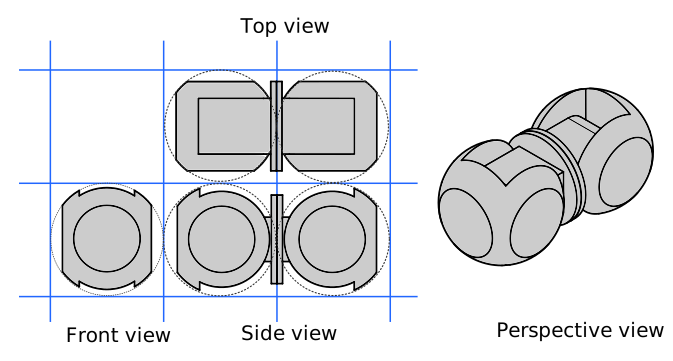
\includegraphics[width=\textwidth]{figures/rofi_reference.pdf}
    \caption{The universal RoFI module. Blue lines specify the grid, dotted
    lines marks spheres in which the module in inscribed. }
    \label{fig:rofi_reference}
\end{figure}

\begin{figure}
    \centering
    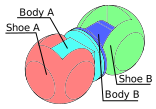
\includegraphics[width=0.7\textwidth]{figures/rofi_body_parts.pdf}
    \caption{Parts of the universal module.}
    \label{fig:rofi_body_parts}
\end{figure}

There are 3 degrees of freedom (figure \ref{fig:rofi_axis}):
\begin{enumerate*}
    \item shoe A can rotate against body A along the $\alpha$ axe in a range
    $\langle -90^\circ; +90^\circ\rangle$,
    \item shoe B can rorate against body B along the $\beta$ axe in a range
    $\langle -90^\circ; +90^\circ\rangle$ and
    \item body A can rotate against body B along the $\gamma$ axe in $\langle
    -180^\circ; +180^\circ\rangle$ with an overflow\footnote{First prototypes
    feature a limitation on a number of overflows in one direction the $\gamma$
    axe due to technical limitations. }.
\end{enumerate*}
The module should be able to provide at least 1.5 $\text{N}\cdot\text{m}$ of
torque for each axe.

\begin{figure}
    \centering
    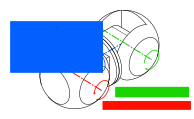
\includegraphics[width=0.7\textwidth]{figures/rofi_axis.pdf}
    \caption{Degrees of freedom of the universal module. The figure represents neutral position of each joint.}
    \label{fig:rofi_axis}
\end{figure}

The flat faces of shoes feature docking system for establishing mechanical
connection to other modules. There are 6 docks in total (figure
\ref{fig:rofi_locks}); 3 on each shoe. The docks are marked by the name of a
shoe and by one of following suffixes: $-1$, $0$, $1$. When facing the dock, its
index gives a factor by which we multiply degree of rotation to turn a shoe
around its axe in counter clockwise direction. Each dock is oriented. We denote
the orientation with an orientation vector. The vector starts in a middle of the
dock. The dock orientation is important for describing configurations of a
system (more detail on that can be found in section \ref{sec:configuration}).
Details about docking mechanism are given in section \ref{subsec:lock}.

\begin{figure}
    \centering
    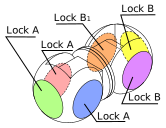
\includegraphics[width=0.7\textwidth]{figures/rofi_locks.pdf}
    \caption{Docks on the universal module. The arrow on each dock specifies its orientation.}
    \label{fig:rofi_locks}
\end{figure}

As it can be seen from the figures \ref{fig:rofi_reference} and
\ref{fig:rofi_body_parts}, the module does not occupy the whole space provided
by the grid. The module is (nearly) inscribed to two spheres (marked by a dotted
line in the figure \ref{fig:rofi_reference}). This allow the module to move its
shoe even if all neighbouring grid cells are occupied. We refer to this property
as \emph{grid-awareness}. This allows the module reconfigure more easily in
densely occupied grid -- see figure \ref{fig:grid_aware} for an example of such
a situation. Another perspective on grid-awareness of the universal module is
that no matter what position it is in, it never outreaches shape specified in
the figure \ref{fig:rofi_grid}.

\begin{figure}
    \centering
    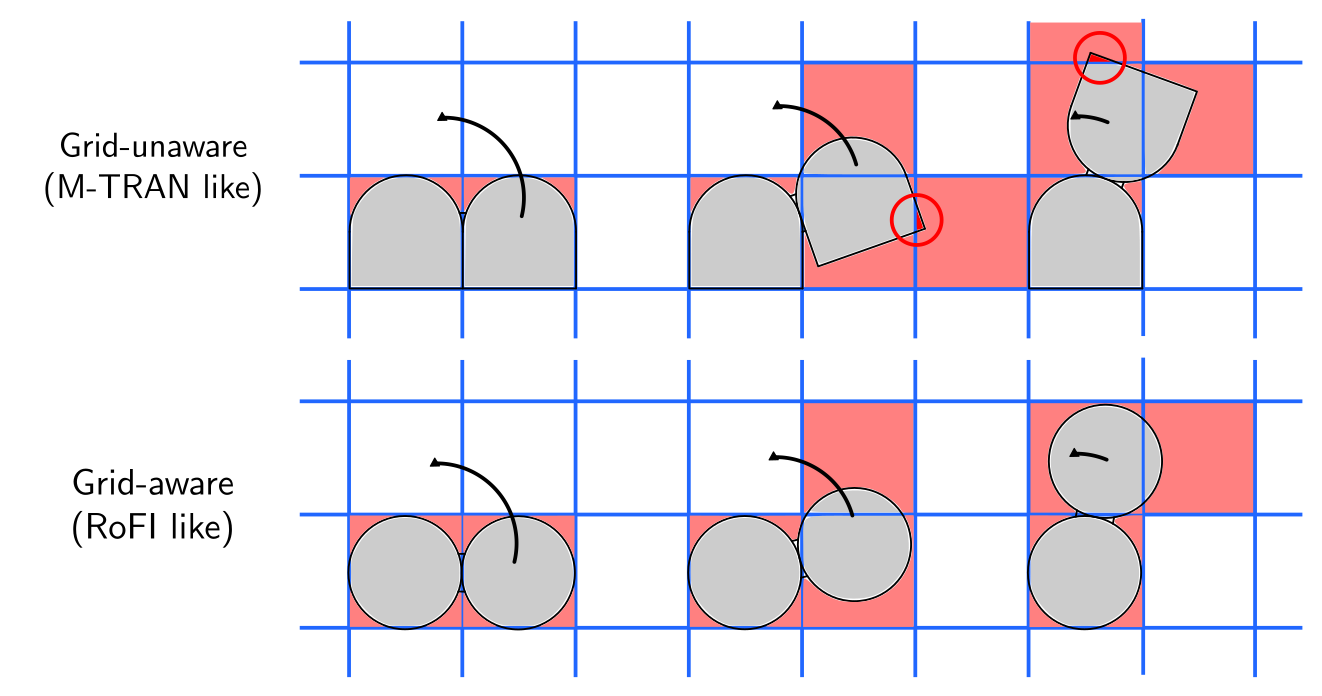
\includegraphics[width=\textwidth]{figures/grid_aware.pdf}
    \caption{Visualization of grid-awareness. Consider two module shapes -- M-TRAN\cite{haruhisa_kurokawa_m-tran_2003}
     like (int the top row) and RoFI like (in the bottom row). Given the task to
     move right body over the left one, M-TRAN like module occupies extra cells
     due to small parts of it body overlapping out of the gird. On the other
     hand, RoFI like module occupies the least cells required to make the
     movement.   }
    \label{fig:grid_aware}
\end{figure}

\begin{figure}
    \centering
    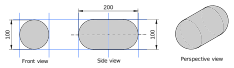
\includegraphics[width=\textwidth]{figures/rofi_grid.pdf}
    \caption{Reference shape for grid-awareness. If the module can be always inscribed in the shape, it is grid-aware.}
    \label{fig:rofi_grid}
\end{figure}

The grid-awareness prevents a face to face contact between two universal
modules. If the modules dock directly face to face, they would not fit in grid.
If the modules fully utilize the space allowed by the reference shape (figure
\ref{fig:rofi_grid}), they would feature only a point contact as two spheres
have only a single point touch. Therefore, there is a need for retractable
docking system. The docking system is specified in section \ref{subsec:lock}.
Here we only describe its relation to the grid.

If the module does not dock with another module, the dock is retracted in the
module shoe and therefore, the module does not outreach the reference shape.
When two modules dock to each other, the docks expand and connect to each other.
As the modules are now connected and no motion between them can be performed,
the enlarged footprint of module over the reference shape does not matter.
Illustration of the docking process can be found in the figure
\ref{fig:rofi_locking_example}.

\begin{figure}
    \centering
    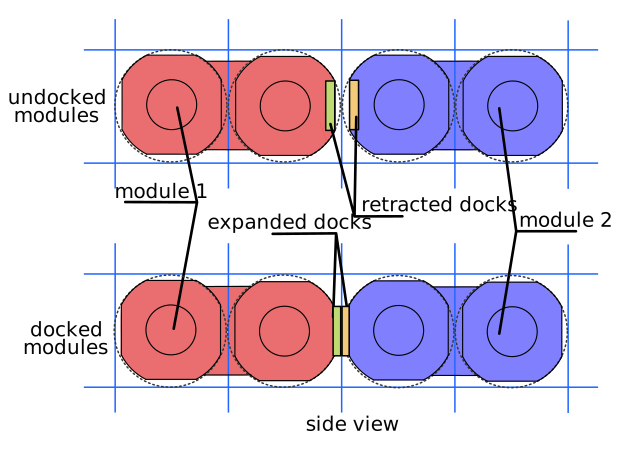
\includegraphics[width=\textwidth]{figures/rofi_locking_example.pdf}
    \caption{Docking procedure. There is a by-default retracted docking system
    in the module which expands when the docking should be performed.}
    \label{fig:rofi_locking_example}
\end{figure}

\subsection{Defining Custom Modules}\label{subsec:custom_modules}

\subsection{Docking System}\label{subsec:lock}

\subsection{RoFI Configuration and Capabilities} \label{sec:configuration}

To ease and unify the development of a firmware and reconfiguration algorithms,
we give means to describe the system made out of RoFI modules. First, there is
a globally unique ID (\emph{GUID}) assigned to each module. GUID is a 128-bit
number. Second, when talking about RoFI systems, we distinguish two terms:
\emph{topology} and \emph{configuration}: \todo{or configuration and realisation?}

\paragraph{topology} Intuitively, topology describes the connection between the
modules in a system and does not care about physical layout of the modules.
Formally, we define it as an undirected graph, where:
\begin{itemize}
    \item nodes are labeled by module GUIDs. There is exactly one node for each
    module in the system.
    \item edges represent a connection two docks. The edge is labeled by a pair
    describing the connection. For modules with GUIDs $a$ and $b$, connection by
    docks $d_a$ and $d_b$ in an orientation $o$ the label is: $(o, \{(a, d_a),
    (b, d_b)\})$. There is at most one edge for each dock on the module. The
    orientation of docks is defined further in the text. Note that undirected
    edges enforces that both modules has to actively participate on a
    connection.
\end{itemize}
\todo{Give an example (text + figure)}

\paragraph{configuration} Intuitively, configuration is a topology with the
actual module positions. Formally, it is a pair $(G, L)$, where $G$ is a
topology and $L: \text{GUID} \rightarrow \text{Axis} \rightarrow \mathcal{R}$ is
a function giving us position of each axis of each module.

As we mentioned in sections \ref{subsec:universal_module} and \ref{subsec:lock},
each dock features an orientation vector. When two docks connect, their
orientation vectors can hold angle of $0^\circ$, $90^\circ$, $180^\circ$ or
$270^\circ$ (measured counter clockwise from a perspective one of the modules
from shoe center to the dock center). Notice, that the angle is the same no
matter which module we choose. Therefore, we give a following convention for the
orientation:

If we aim one of the orientation vectors up (to the \emph{north}), the other
vector aims either:
\begin{enumerate*}
    \item \emph{north},
    \item \emph{east},
    \item \emph{south} or
    \item \emph{west}
\end{enumerate*}
as shown on figure \ref{fig:dock_orientation}.
Therefore we define the orientation $o$ to be an element of $O = \{N, E, S,
W\}$.

\begin{figure}
    \centering
    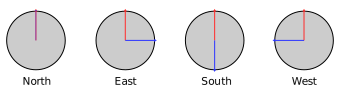
\includegraphics[width=\textwidth]{figures/dock_orientation.pdf}
    \caption{Possible orientation of two dock. Orientation vector of current
    perspective is shown as red, the orientation vector of mating dock is shown
    as blue. Note that it during a connection, it does not matter which dock's
    perspective we choose.}
    \label{fig:dock_orientation}
\end{figure}

We define a \emph{model} $M = (V, D)$ of an configuration. $V$ is set of spheres
in 3D space over-approximating shape of the modules in a system. $D$ is a set of
named orientation vectors of all docks in the system positioned in space. Both
$D$ and $V$ can be computed via transformation matrixes build from axis
orientation and knowledge of module geometry.

We call a configuration $C = (G, L)$ with \emph{realizable} iff:
\begin{enumerate}
    \item no two spheres in $D$ intersects and
    \item for each two docks that are connected in $G$:
        \begin{enumerate}
            \item their orientation agrees with orientation in $L$,
            \item their origin points are the same and
            \item the plane defined by their orientation vectors is perpendicular to axis of a dock.
        \end{enumerate}
\end{enumerate}
Note, that there are no constraints on topology and we consider every topology
as valid. However, for some topologies there exists no possible configuration.
\todo{Give example of possible configuration, impossible due to both factors}

\subsection{Intermodule Communication and Power Sharing}

\subsection{Intramodule Architecture}

\subsection{The RoFI "BIOS" \todo{Proper naming}}

\subsection{RoFI lib}

\todo{Something here}